\section{Writing Tool}
\label{prototype:WritingTool}
Having refocused my development efforts back towards producing a self-built tool for note writing I built this prototype using Fabric JS -  the same tool used to build my \nameref{prototype:WebDrawing} (but with a more complex implementation)


Although this took a couple of hours to build, I found the problem-solving workflow both enjoyable and satisfying.

Whilst building the system I explored some areas of web development new to me: preventing default browser handling of click / trackpad integration to enable my custom scrolling/zooming/panning action on the drawing surface.

Whilst I have only integrated written interaction so far, I included a text box to demonstrate the flexibility I can build in. users will soon be able to add shapes, annotate images, have full typing tools and so much more as I iterate on this primitive first design.

My database was also modified to hold the note data enabling the user to recall their different files by clicking the note 'node' from the map view

Whilst I am very happy with the laptop / desktop experience of note editing (primarily regarding the interactions possible around the canvas), there Is still work to do on the touchscreen interactivity of this element. While it is registered (and the image moves), there is occasionally issues with highlighting, page freezing etc which I need to solve. I was pleased to find pre-existing tools - https://excalidraw.com - which has solved these challenges on iPad, therefore showing it is possible

\subsection*{Version 1:}
the image below is from a version integrated into my mind map (as referenced in my diary - this part of the software can easily be substituted for a linked OneNote page should the user wish to do so)


\begin{figure}[H]
\centering
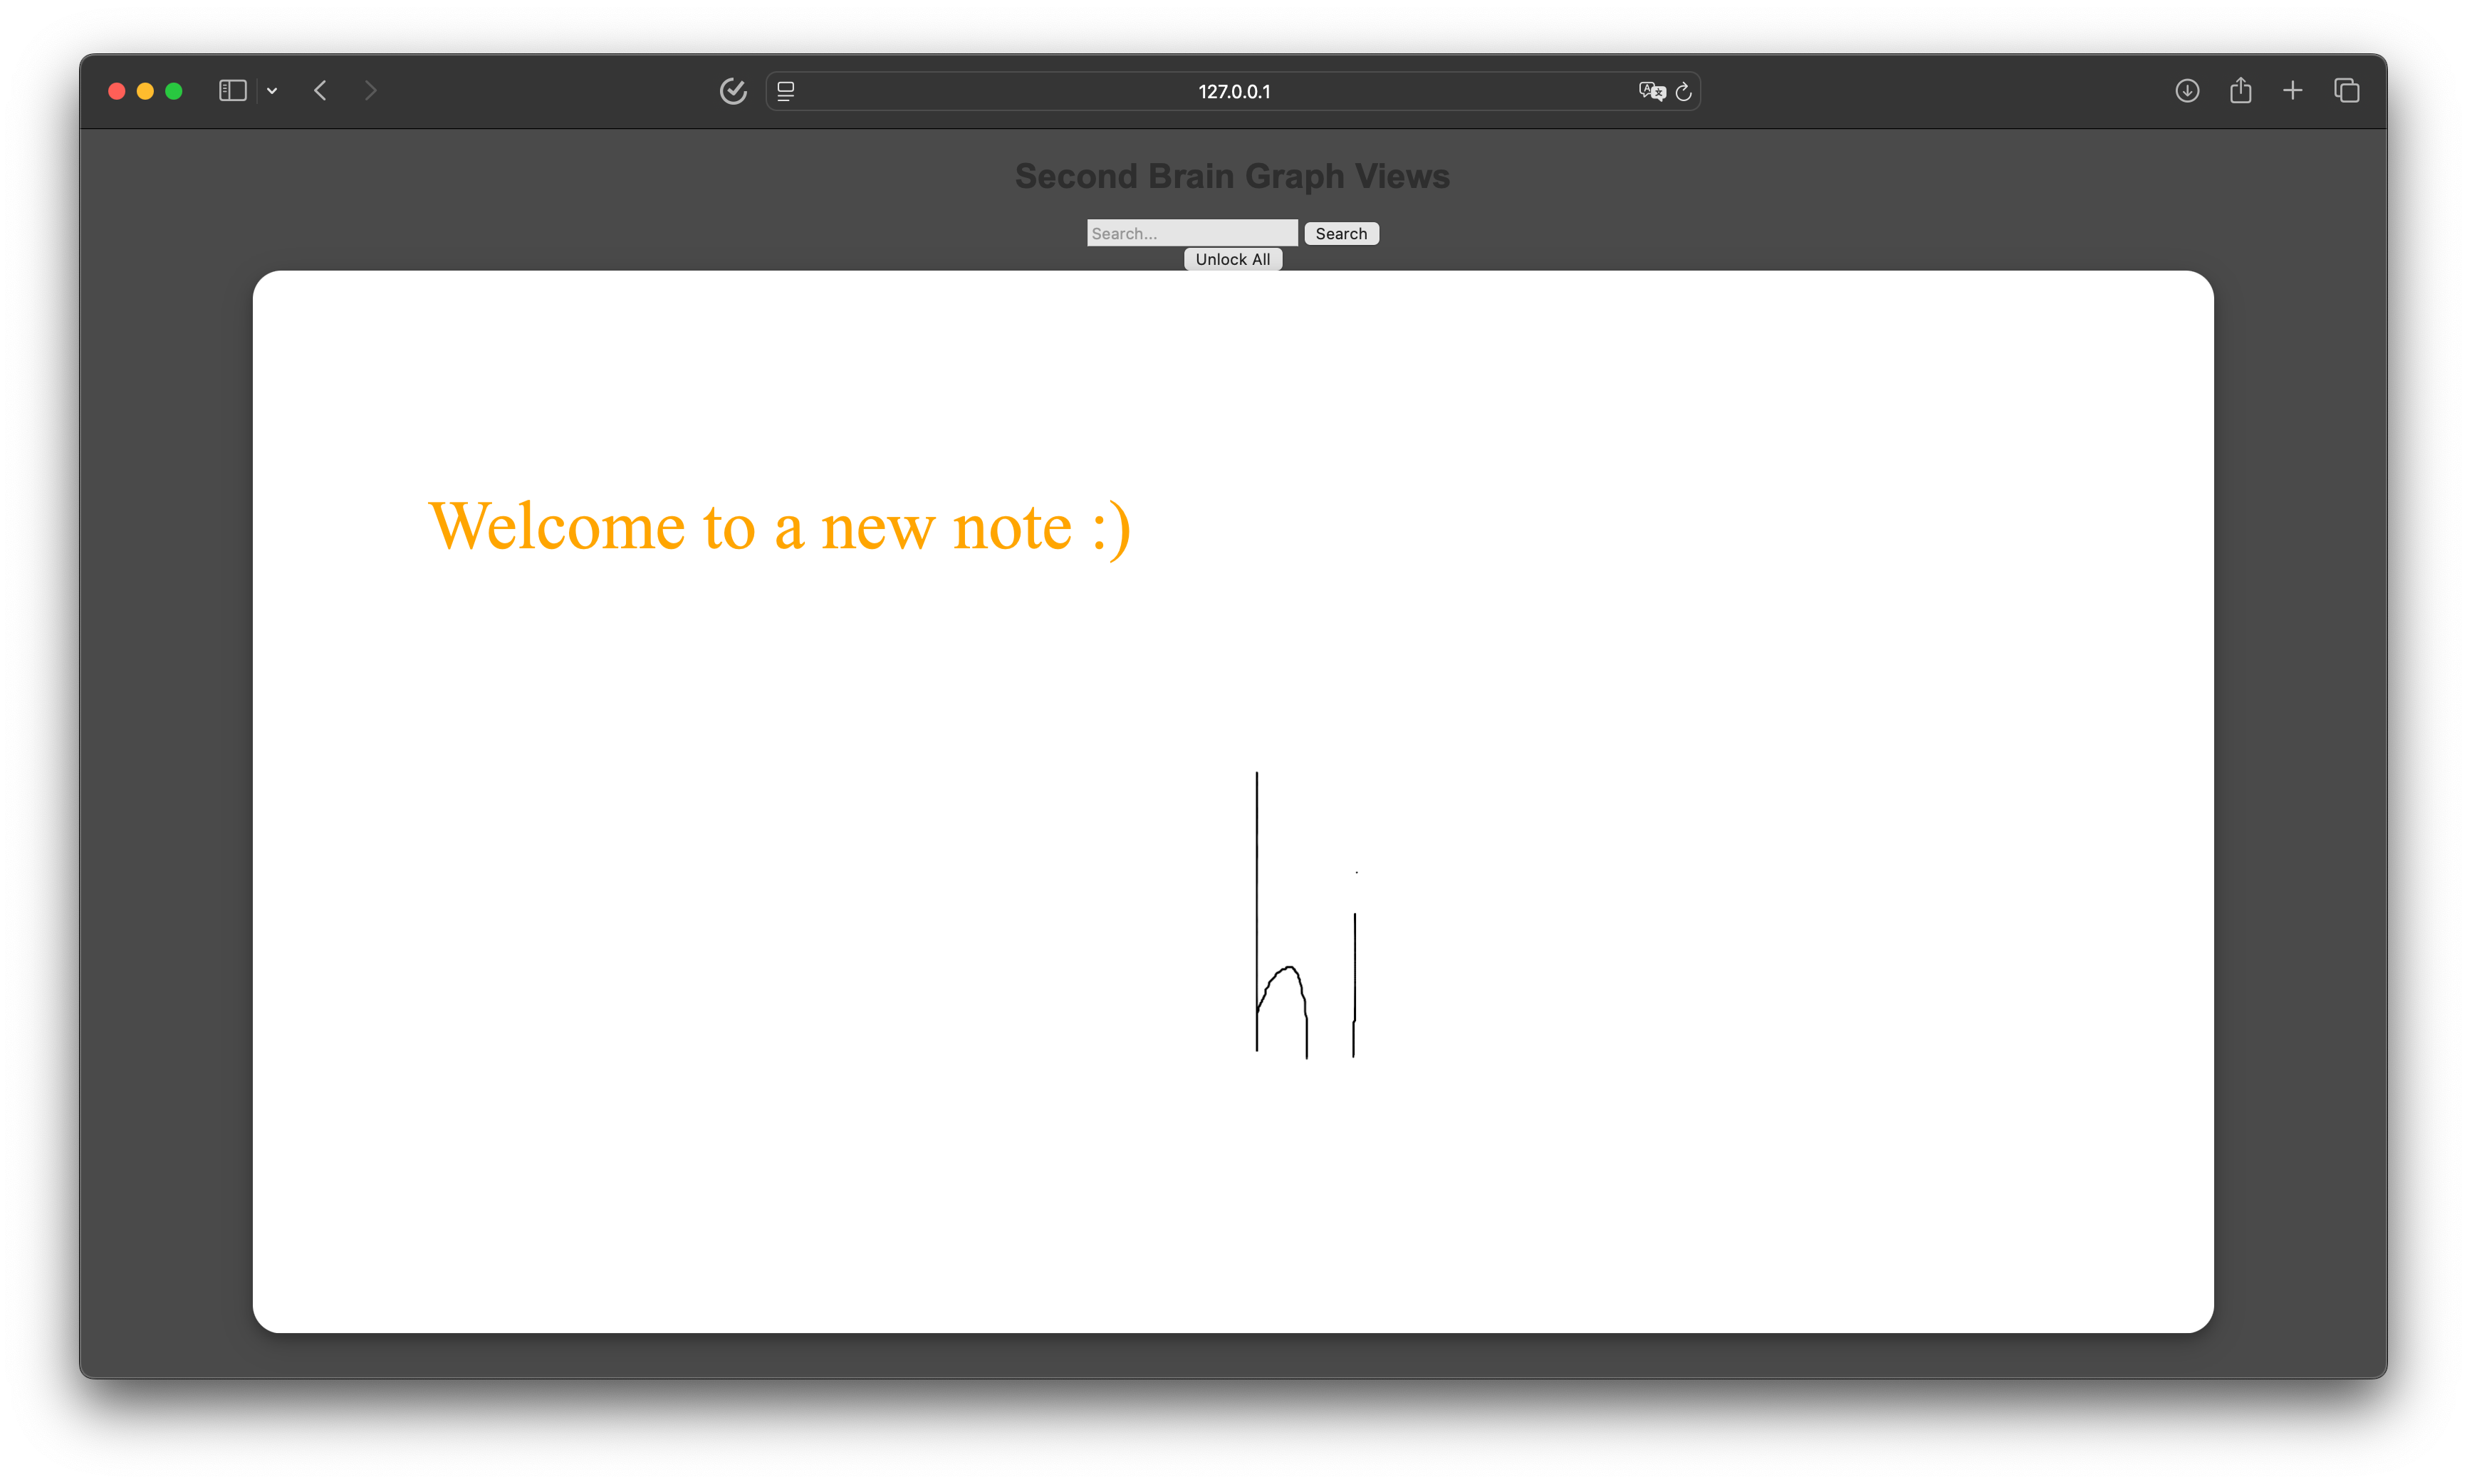
\includegraphics[width=0.8\textwidth]{Prototype/10_WritingTool/media/prototype1.png}
\caption{My note writing tool prototype}
\end{figure}

\subsection*{Version 2:}
Update: 

Having found some more spare time I have continued working on my note writing system. Thanks to my thorough prior research into creating a robust and well architected canvas system the addition of many features was possible in a short period of time.

Within 2 hours of work I have now added the ability to:
\begin{itemize}
	\item Rename notes within the editor
	\item Toggle between text and drawing mode for typing / handwriting
	\item Add simple shapes (a system I want to build out to include diagram elements, tables and sticky notes)
	\item Add text boxes for typing (I want to create a simpler way to start typing though without this click)
	\item Pen colour picker (which uses the native system / browser API to ensure maximum usefulness - e.g larger desktop displays will show more detail whereas iPad displays are a simpler colour wheel)
	\item Pen width adjustments
	\item Background changing options (this took the longest to implement and required creating a secondary patterned canvas underneath the standard drawing/typing canvas, and then matching the movement such as panning
	\item Ability to delete notes from within the editing screen (though I might remove this option / add a confirmation prompt to prevent unintended activations)
\end{itemize}

\begin{figure}[H]
\centering
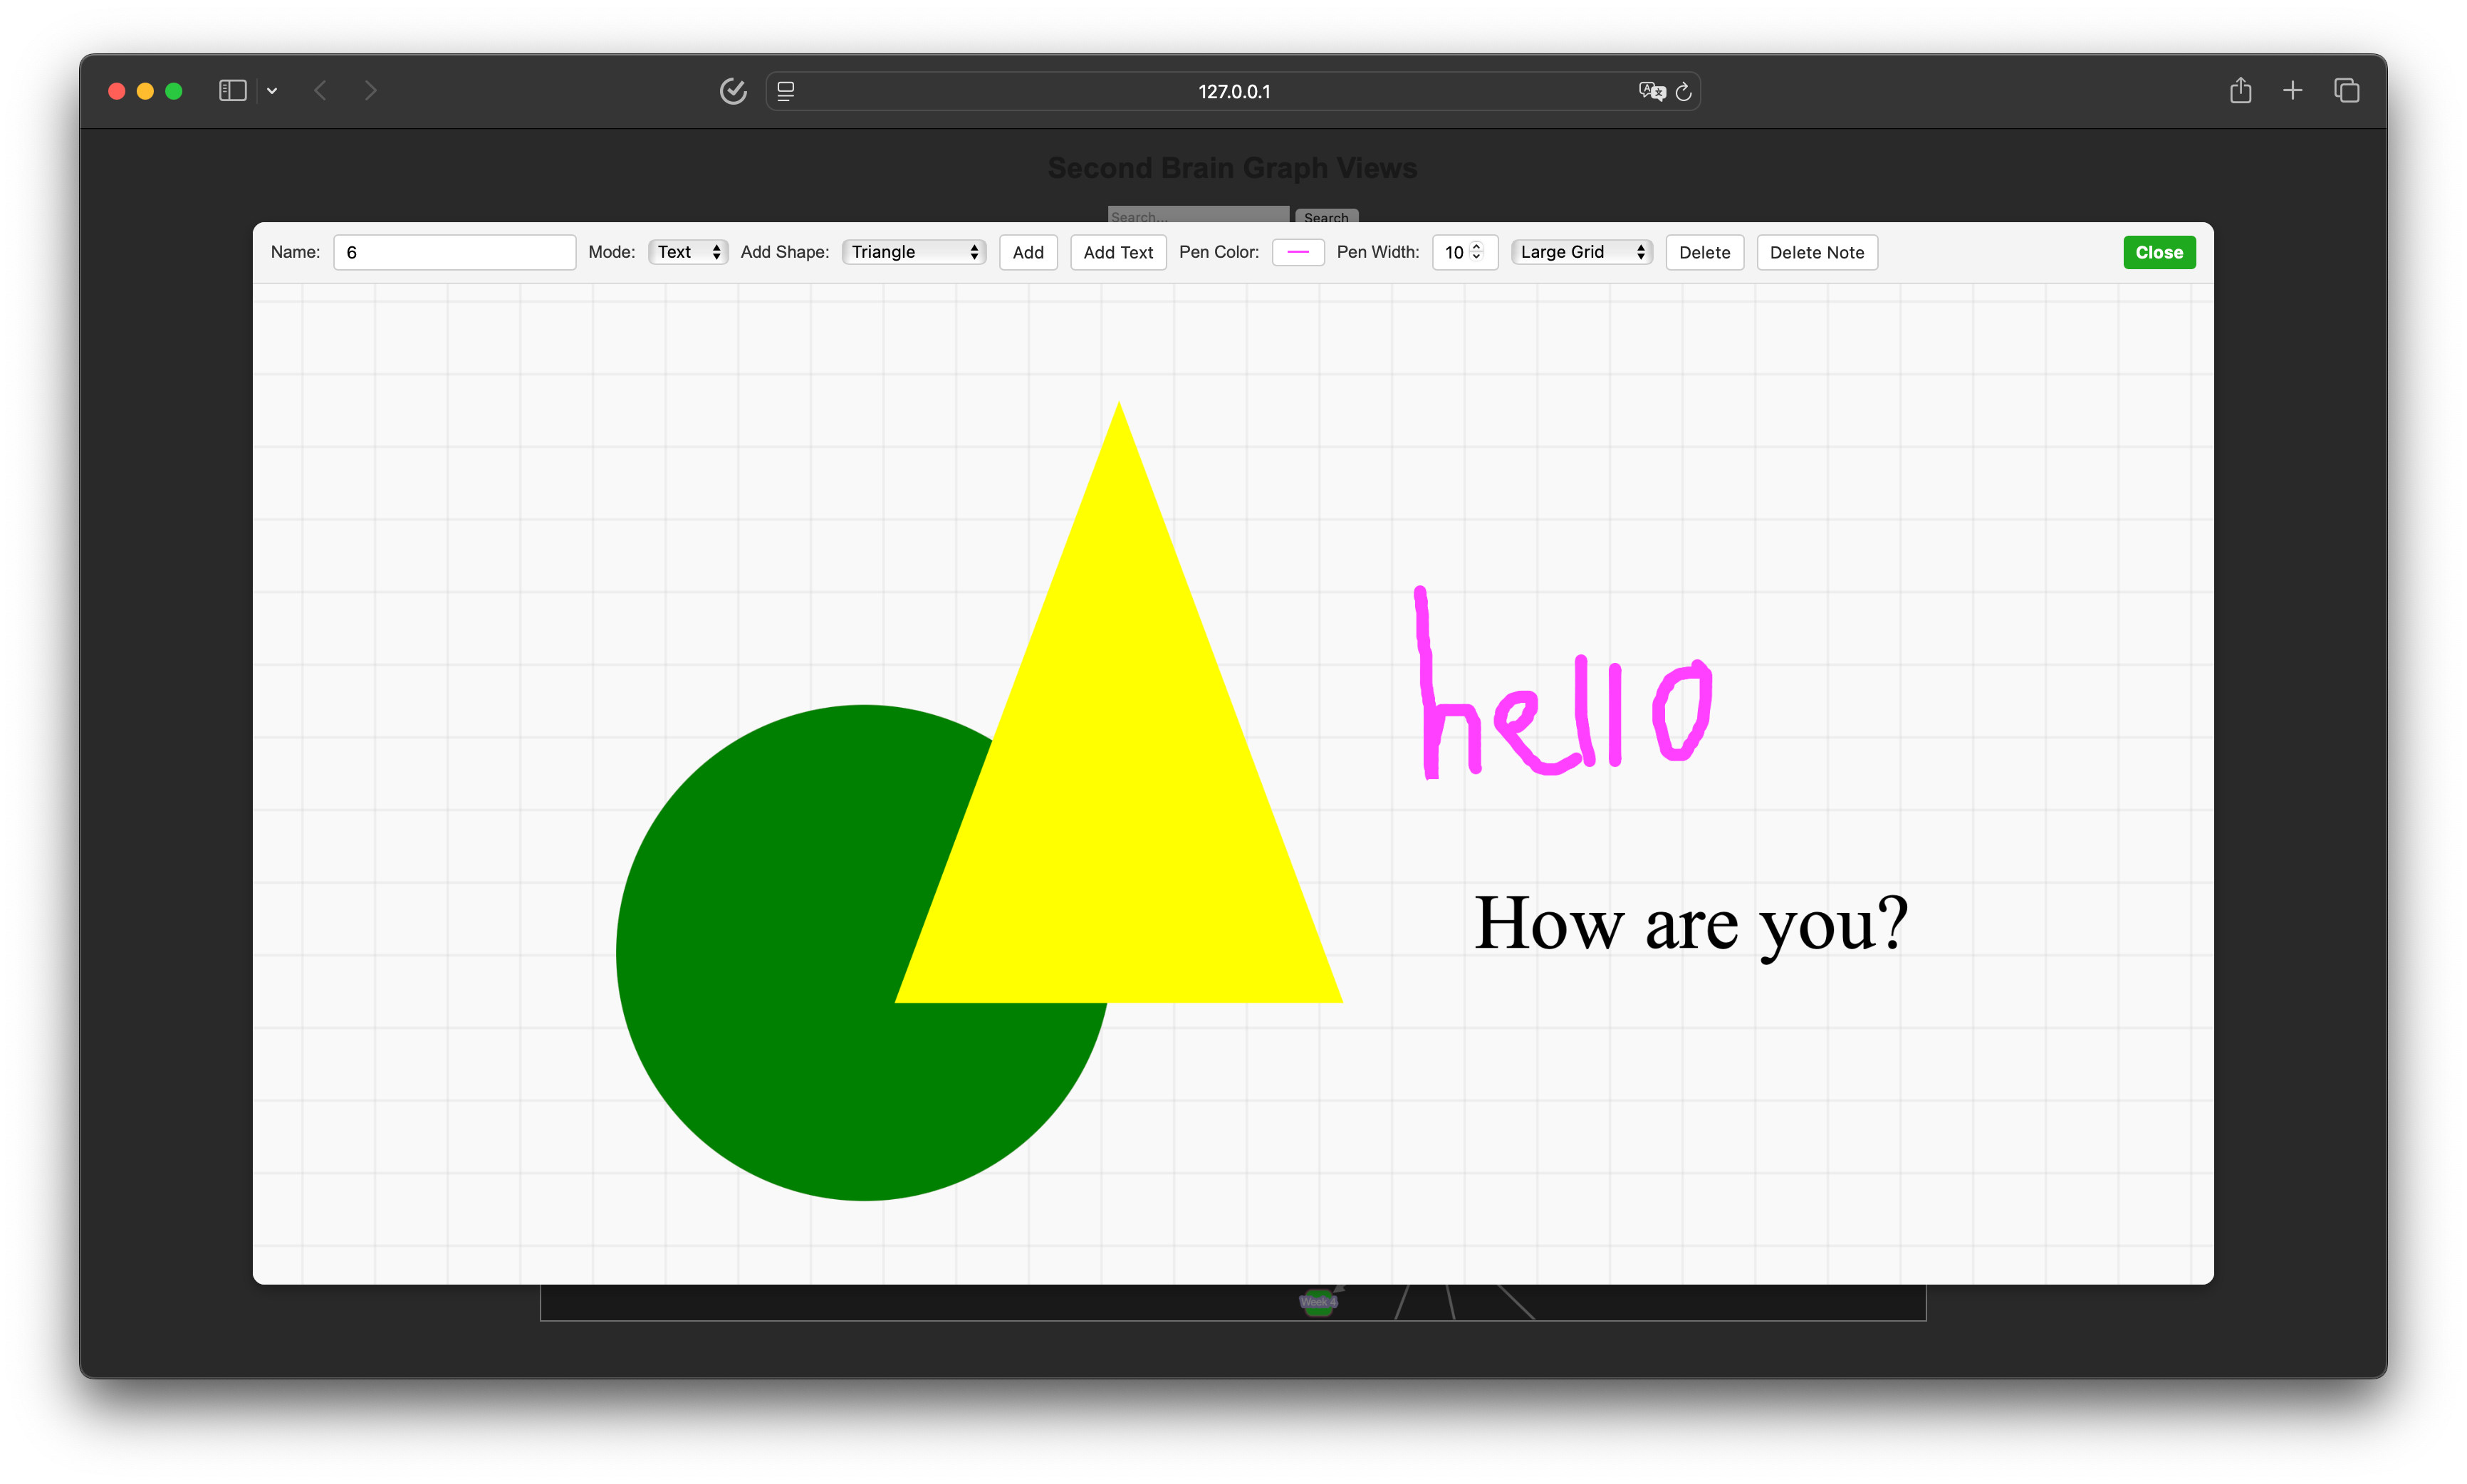
\includegraphics[width=0.8\textwidth]{Prototype/10_WritingTool/media/prototype2.png}
\caption{My note writing tool prototype with new features}
\end{figure}    


